\documentclass{article}

\usepackage{amsmath}
\usepackage{graphicx}
\usepackage{geometry}
\usepackage{float}
\usepackage{subfig}

\newcommand{\W}{{\mathcal W}}

\title{Numerical simulation of the shallow water circular hydraulic jump}

\author{
    David I. Ketcheson \and
    Manuel Quezada de Luna
}
\begin{document}

\maketitle

\begin{abstract}
We study numerical discretizations of the shallow water equations
for the simulation of the circular hydraulic jump formed
when a vertical fluid jet impacts a horizontal plate.  
We test a range of numerical methods, including finite volume Godunov-type
methods with a variety of approximate Riemann solvers, and
a continuous Galerkin finite element method based on flux-corrected transport (FCT).
The finite volume methods are employed on a uniform cartesian grid
while the finite element method uses an unstructured triangular grid.
The methods give completely different results, even for highly-refined meshes.
\end{abstract}


\section{Introduction}

\subsection{The circular hydraulic jump}

Perhaps the first reference to the observation of the circular hydraulic jump
comes from Lord Rayleigh \cite{rayleigh1914theory}, who wrote that it
``may usually be seen whenever a stream of water from a tap strikes a horizontal
surface".  This phenomenon that is familiar in the everyday kitchen sink, is in
fact highly nonlinear and complex.  Near the jet, the flow is shallow and
supercritical, while further away it is deeper and subcritical.  The transition from supercritical
to subcritical flow
occurs in a very narrow region and takes the form of a \emph{jump} or \emph{bore}
that is roughly circular if the surface is flat; we refer to it herein as a
circular hydraulic jump (CHJ).

Early experimental work on the CHJ began some time later
\cite{kurihara1946hydraulic,tani1949water,watson1964radial}.
Watson \cite{watson1964radial} derived the jump radius
implied by Rayleigh's approach and the vertical
velocity profile in the supercritical region, assuming a no-slip
boundary condition at the bottom.  He also studied the turbulent
flow case and performed experiments.
More detailed experiments revealed different qualitative classification
of jumps  \cite{ishigai1977heat,craik1981circular}.
Although later work incorporated more physical details (such as surface tension) into the models
\cite{bush2003influence}, Bohr et. al. showed that important properties of the jump
(particularly its radius) could be reasonably predicted using a simple shallow water
model \cite{bohr1993shallow}.

While the jump is roughly circular, under appropriate conditions it may deviate
from this shape and deform rapidly and chaotically in time.
Instability of the jump was observed from fairly early on \cite{craik1981circular}.
Under special circumstances with more viscous fluids, the jump instability may lead to
the formation of curious shapes such as polygons \cite{ellegaard1998creating}, but
for a low-viscosity fluid like water the behavior is generally chaotic.
The strength of the instability increases with the jet velocity and with the
depth at the outside of the jump.  The flow can be stable for sufficiently small
velocities and depths.

\subsection{Scope of this work}
This work is intended to be more exploratory than explanatory; in other words,
it is focused more on raising significant questions than on answering them.
The central issue is the stability of the shallow water CHJ, from both a
physical and a numerical perspective.
The main result is our finding that a number of numerical methods that are
in use give completely different solutions to the CHJ problem.
These differences do not diminish when the grid is refined.
Evidence suggests that, at least in some regimes, the CHJ is unstable
and solutions are chaotic.  This implies that one should not expect pointwise
convergence of solutions, so a traditional study of accuracy of the numerical
methods is ruled out.

\subsection{Numerical shock instabilities}

In \cite{peery1988blunt} a numerical instability was observed to
appear near the symmetry plane in the simulation of a bow shock.
This phenomenon, known as a ``carbuncle", has been observed by many researchers
in similar numerical experiments for the Euler equations, and many remedies
have been proposed, mainly in the form of additional numerical dissipation
\cite{quirk1997contribution,pandolfi2001numerical,dumbser2004matrix,chauvat2005shock,ismail2009proposed,shen2014stability}.
Most notably, the HLLE Riemann solver suppresses the carbuncle instability \cite{quirk1997contribution}.
For a recent review of numerical shock instability and work to alleviate it,
we refer to \cite[Section 2.5]{simonnumerical}.

Given the similarity of structure between the Euler equations and the shallow
water equations, one might expect carbuncles to appear in numerical
solutions of the latter as well.  Indeed, this has been observed \cite{kemm2014note}.
The shallow water carbuncle behaves in a fashion very similar to the
Euler carbuncle: it appears when the Roe solver is used, but not when
the HLL solver is used, and at least some of the other methods that suppress
the latter also suppress the former \cite{kemm2014note,bader2014carbuncle}.

Meanwhile, some research has suggested that the carbuncle is not purely a
numerical instability but instead is the manifestation of a true physical
instability \cite{moschetta2001carbuncle,elling2009carbuncle}.

The carbuncle has not previously been observed in circular hydraulic jump
simulations.  However, it is known to appear in the presence of steady shocks
that are nearly aligned with the grid, so it is natural to expect it, and as we
will see it does indeed arise.  Its presence is particularly interesting 
in this circumstance since there is a known physical instability that affects
the shock.  A natural question is whether the carbuncle in this instance is
a purely numerical phenomenon or a manifestation of the physical instability.

\section{The shallow water circular hydraulic jump}
The shallow water equations in two (horizontal) dimensions are
\begin{subequations} \label{eq:sw}
\begin{align}
    h_t + (hu)_x + (hv)_y & = 0 \\
    (hu)_t + \left(hu^2 + \frac{1}{2}gh^2\right)_x + (huv)_y & = 0 \\
    (hv)_t + (huv)_x + \left(hv^2 + \frac{1}{2}gh^2\right)_y & = 0.
\end{align}
\end{subequations}
These can be written in vector form as
\begin{align}
    q_t + f(q)_x + g(q)_y & = 0.
\end{align}

\subsection{Semi-analytical steady solution under rotational symmetry}

By assuming rotational symmetry in \eqref{eq:sw}, one obtains the
system (in one spatial variable)
\begin{subequations} \label{eq:rsw}
\begin{align}
    (rh)_t + (rhu)_r & = 0 \label{mass1} \\
    (rhu)_t + (rhu^2)_r + r \left(\frac{1}{2}gh^2\right)_r = 0. \label{mom1}
\end{align}
\end{subequations}
Steady-state solutions of \eqref{eq:rsw} satisfy
\begin{subequations}
\begin{align}
    rhu & = C \\
    h'(r) & = \frac{h}{\frac{g}{\beta^2} r^3 h^3 -r} = \frac{h}{r} \cdot \frac{F^2}{1-F^2} \label{eq:dh}
\end{align}
\end{subequations}
for some $C$ independent of $r$.  Here $F=|u|/\sqrt{gh}$ is the Froude number.
We see that two types of steady profiles exist, depending on whether the flow
is subcritical ($|F|<1$) or supercritical ($|F|>1$).  No smooth steady solution can
include both regimes, since the right hand side of \eqref{eq:dh} blows up when $F=1$.

The steady, rotationally-symmetric circular hydraulic jump involves supercritical
flow for $r<r_0$ and subcritical flow for $r>r_0$, where $r_0$ is the jump radius.
The jump itself takes the form of a stationary shock wave.  The Rankine-Hugoniot jump
conditions specify that for such a shock,
\begin{align} \label{eq:RH}
    h_+ - h_- & = \frac{-3h_- + \sqrt{h_-^2 + 8 h_- u_-^2/g}}{2} = \frac{3h_-}{2}\left(\sqrt{1+\frac{8}{9}(F_-^2-1)}-1\right),
\end{align}
where the subscripts $+, -$ denote states just inside or outside the jump radius, respectively.

A steady-state, rotationally symmetric solution can be given for an annular region as follows:

\begin{enumerate}
    \item Specify the depth and velocity at the inner boundary (near the jet) and outer boundary.
    \item Integrate \eqref{eq:dh} from both boundaries.
    \item Find a radius $r_0$ where the matching condition \eqref{eq:RH} is satisfied.
\end{enumerate}
Due to the nature of solutions of \eqref{eq:dh}, it can be shown that the required jump
radius $r_0$ always exists if the prescribed flow is supercritical at the inner boundary
and subcritical at the outer boundary.

Numerical tests suggest that the solution obtained in this way is a stable equilibrium
of the reduced one-dimensional shallow water equations \eqref{eq:rsw}.  This
solution provides a useful starting point for testing the stability of the CHJ
as a solution of the full two-dimensional shallow water equations \eqref{eq:sw}.

\section{Numerical methods}

Potential methods to try:
\begin{itemize}
    \item Galerkin methods on cartesian grids (to see if carbuncles appear)
    \item FV methods on perturbed grids (to avoid grid alignment)
    \item FV methods on annular grids (with grid alignment everywhere)
    \item Various Riemann solvers intended to avoid carbuncles
\end{itemize}

\subsection{Finite volume methods}

\subsubsection{Roe solver}

\subsubsection{HLLE (2-wave) solver}
The HLLE solver approximates the Riemann solution using two waves with
speeds $s_1, s_2$.  The middle state is
\begin{align} \label{qm-HLL}
    q_m^\textup{HLLE} = \frac{f(q_l) - f(q_r) + s_2 q_r - s_1 q_l}{s_2 - s_1}.
\end{align}


\subsubsection{A 3-wave solver}
Refinements of the HLLE solver were subsequently introduced in order to better
resolve contact and shear waves, which are strongly dissipated by the HLLE solver.
In the shallow water equations, we have only a shear wave.  We can introduce a third
wave in the approximate Riemann solver that carries the jump in the transverse velocity.
For simplicity, we describe this solver for an x-interface; i.e. where $u$ is the normal
velocity component and $v$ is the tangential velocity component.  Then the Riemann
solution is assumed to consist of 3 jump-discontinuities $\W^1, \W^*, \W^2$ where $\W^{1,2}$
carry all of the jump in $h$ and $hu$ while $\W^*$ carries all of the jump in $hv$.

The values $h_m$ and $u_m$, along with the speeds for the waves $\W^1,\W^2$ 
are thus determined by the same formula \eqref{qm-HLL} as in the HLL solver.
The speed of the middle wave is determined by conservation:
$$
    s^* = \frac{h_r u_r v_r - h_l u_l v_l}{h_r v_r - h_l v_l}.
$$
The middle state transverse velocity $v_*$ is given by $v_l$ if $s^*>0$ or $v_r$ if $s^*<0$.

\subsubsection{HLLEMCC solver}
The HLLEMCC approximate Riemann solver for the shallow water equations was proposed
in \cite{kemm2014note} specifically to deal with carbuncles.  The idea is to adjust
the amount of dissipation applied to the shear wave, adding dissipation in regions
where unphysical carbuncles would appear.  The approximate solution in this
case consists of four waves; the faster waves use the HLLE wave speeds and carry
jumps only in the depth and normal momentum, while the slower waves carry jumps
only in the transverse momentum.  By adjusting the value of $\phi$, this solver
can behave like the HLLE solver (if $\phi=1$) or like the Roe solver (if $\phi=0$).

The middle states $q^1_m, q^2_m$ are the same as those used for the HLLE solver.
Requiring conservation of the transverse momentum gives
$$
    q^3_m = \frac{f^3_l - f^3_r - (\hat{v}-\phi\hat{c})q^3_l + (\hat{v}+\phi\hat{c})q^3_r}{2\phi\hat{c}}.
$$
Here $\hat{v}, \hat{c}$ are the Roe-average normal velocity and sound speed, respectively, whereas the function $\phi$ is given by

\begin{equation}\label{if}
\phi(\theta)=min\left\lbrace 1,\, \left(\varepsilon\,\theta\,max\left\lbrace0,\,1-Fr_{u}^{\alpha} \right\rbrace \right)   \right\rbrace^{\beta}
\end{equation}

where $Fr_{u}$ is the Froude number perpendicular to the cell face and $\varepsilon$, $\alpha$, and $\beta$ are parameters that have to be chosen appropriately. For the shallow water equations, authors in \cite{kemm2014note} propose to use $\varepsilon=10^{-3}$ and $\alpha=\beta=\frac{1}{3}$. The value of $\theta$ is calculated as the 2-norm of the residual in the Rankine-Hugoniot condition for the shear wave.\\

The HLLEMCC solver follows the ideas of the Harten-Hyman entropy fix by splitting the shear wave with speed $\hat{u}$, into two waves moving with speeds $\hat{u}-\phi\hat{c}$ and $\hat{u}+\phi\hat{c}$ (see figure \ref{HLLEMCC}). Its implementation, in terms of the fluctuations, is performed by using the values $\hat{u}^{\pm}$ calculated with an absolute-value function defined as

\begin{equation}\nonumber
\varphi(\lambda)=\frac{\vert \lambda-\phi(\theta)\hat{c}\,\vert+\vert \lambda+\phi(\theta)\hat{c}\,\vert}{2}
\end{equation}

\begin{figure}
    \center
    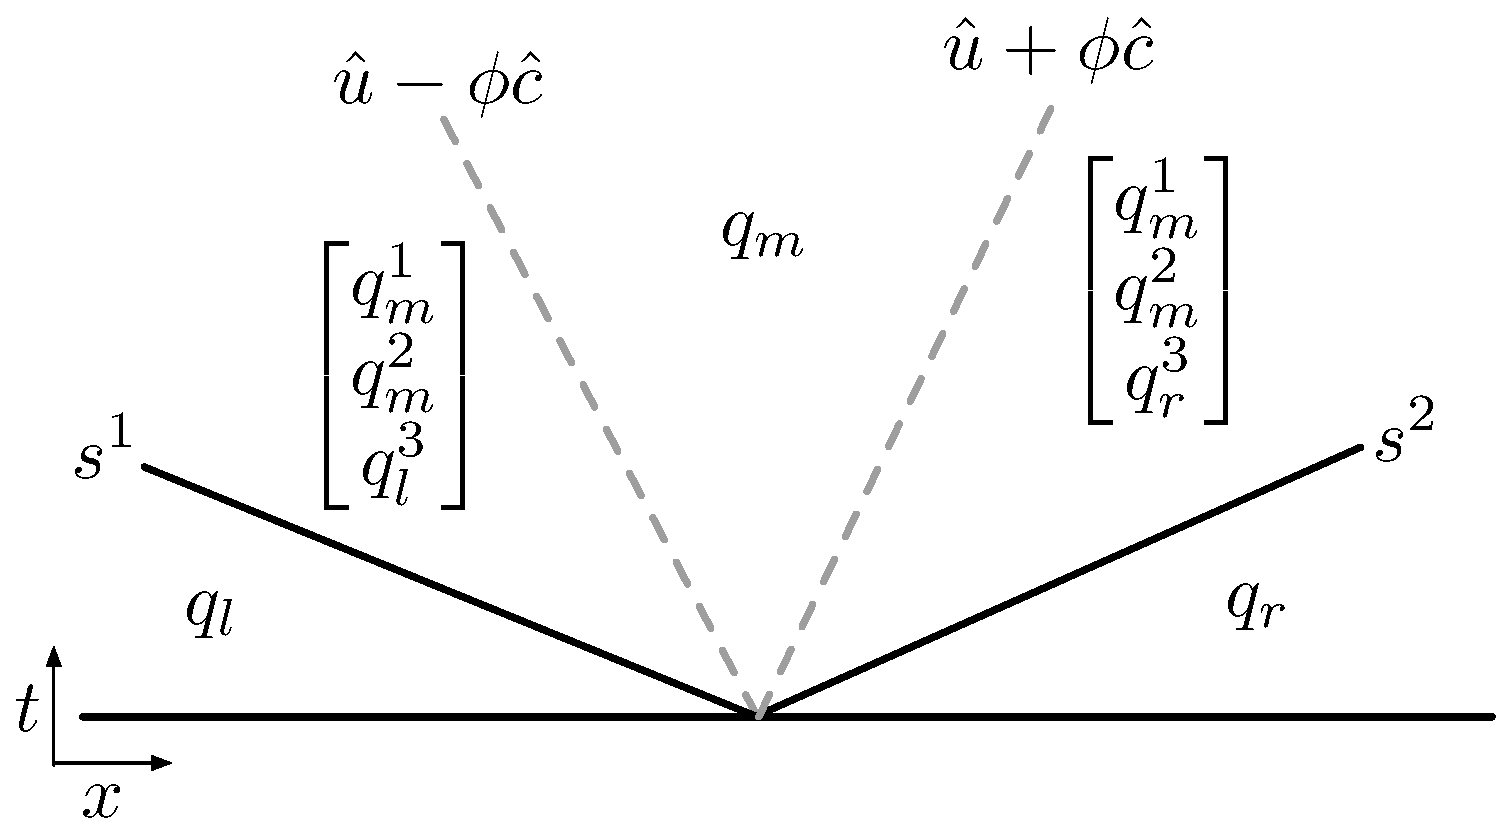
\includegraphics[width=0.6\textwidth]{figures/hllemcc.pdf}
    \caption{Structure of the HLLEMCC approximate Riemann solution, with four waves.}
    \label{HLLEMCC}
\end{figure}

\subsection{Continuous Galerkin method}

\subsection{Discontinuous Galerkin method}

\section{Numerical results}

To demonstrate the range of qualitative solutions that can arise when using
different numerical methods, we apply several schemes to the following setup.
We take
\begin{align*}
    r_0 & = 0.1 & h_0 & = 0.5 & u_0 & = 0.75 \\
    g & = 1 & h_\infty & = 0.15 & F_\infty & = 0.1
\end{align*}
where $r_0, h_0, u_0$ are the jet radius and the depth and velocity at the outer
edge of the jet, respectively; $h_\infty$ and $F_\infty$ are the depth
and Froude number (infinitely) far away from the jet.  The domain is $[-1,1]^2$
and boundary conditions are imposed based on the 1D steady state solution with
the chosen jet and far-field conditions.  The bathymetry is flat and friction is
neglected.  The initial data is chosen to be far from the equilibrium and
consists of a uniform depth of $h=0.15$ and zero velocity.
Results using a $1000\times 1000$ grid are shown in Figure \ref{fig:hlle_vs_roe}.  
We see that by $t=4$, the HLLE solution has already reached the equilibrium
and remains there indefinitely.  In contrast, the Roe solution is highly
unsteady with a very non-circular jump containing cusps that tend to form
near the four points where the jump is aligned with a grid axis.

Based on numerous tests, we have found that results for other initial data
are very similar to those shown here, although of course the details
of the Roe solution differ because the solution is chaotic.

\begin{figure}
  \begin{centering}
    \subfloat[HLLE Riemann solver, t=4]{
      \includegraphics[width=0.45\textwidth]{figures/hlle_1000_t4.eps} 
    }
    \subfloat[Roe Riemann solver with entropy fix, t=4]{
      \includegraphics[width=0.45\textwidth]{figures/roe_1000_t4.eps}
    }

    \subfloat[HLLE Riemann solver, t=20\label{fig:hlle}]{
      \includegraphics[width=0.45\textwidth]{figures/hlle_1000_t20.eps} 
    }
    \subfloat[Roe Riemann solver with entropy fix, t=20\label{fig:roe}]{
      \includegraphics[width=0.45\textwidth]{figures/roe_1000_t20.eps}
    }
  \end{centering}
  \caption{
    Comparison of PyClaw solutions using the classic Clawpack discretization
    with HLLE and Roe Riemann solvers.\label{fig:hlle_vs_roe}}
\end{figure}

Next we apply Kemm's HLLEMCC solver to the same scenario; results are shown
in Figure \ref{fig:hllemcc}.  Results at early times are very similar to
those for the Roe solver.  The cusps that appear have a stronger tendency
to dissipate and then reform, as indicated in the figure at $t=20$.
Nevertheless, they continue to appear indefinitely, based on longer-time
simulations.

\begin{figure}
  \begin{centering}
    \subfloat[HLLEMCC Riemann solver, t=4]{
      \includegraphics[width=0.45\textwidth]{figures/hllemcc_1000_t4.eps} 
    }
    \subfloat[HLLEMCC Riemann solver, t=20]{
      \includegraphics[width=0.45\textwidth]{figures/hllemcc_1000_t20.eps}
    }
  \end{centering}
  \caption{
    PyClaw solutions using the classic Clawpack discretization
    with HLLEMCC Riemann solver.\label{fig:hllemcc}}
\end{figure}

The results above are computed with schemes that include second-order
correction terms.  In Figure \ref{fig:first-order} we compare the corresponding
first-order schemes.  Even by increasing the value of $\epsilon$ to $0.1$,
the carbuncles are not suppressed by the HLLEMCC solver.  Indeed, the Roe
and HLLEMCC solutions look very similar.

\begin{figure}
  \begin{centering}
    \subfloat[Roe Riemann solver, 1st order, t=20]{
      \includegraphics[width=0.45\textwidth]{figures/_1_roe_1000_t20.eps} 
    }
    \subfloat[HLLEMCC Riemann solver, $\epsilon=0.1$, 1st order, t=20]{
      \includegraphics[width=0.45\textwidth]{figures/_1_hllemcc_1000_eps01_t20.eps}
    }
  \end{centering}
  \caption{
    PyClaw solutions using a 1st-order discretization
    with different Riemann solvers.\label{fig:hllemcc}}
\end{figure}



\subsection{Stable jump}

\subsection{Unstable jump}

\section{Conclusions}


\bibliographystyle{apalike}
\bibliography{refs}

\end{document}
